\section{Low-Pass filter}
\label{lowPassFilter}
ADC'en på Arduino UNO's mikroprocessor har en samplingfrekvens på 10k hvor UCN boardet sampler ved 1100. Her kan forekomme alaising og for at undgå dette implementeres et low-pass filter. Et low-pass filter er et filter som sorterer høje frekvenser fra men samtidig tillader DC (jævnstrøm) igennem.


\begin{figure}[h!]
  \centering
  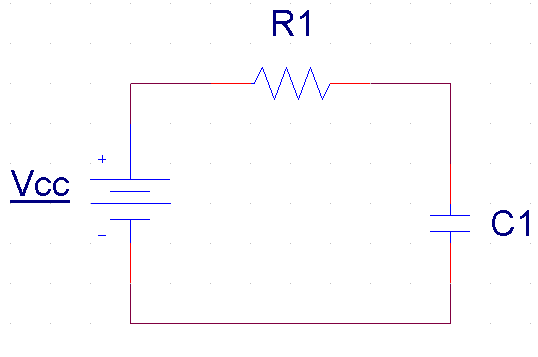
\includegraphics[width=0.6\textwidth]{figures/low_pass_schematic.png}
\end{figure}

Et low-pass filter kan konstrueres med en modstand og en kondensator i serie. Kondensatoren er forbundet til stel så den skaber en AC-kortslutning (vekselsstrøm) og derved filtrer AC væk fra signalet. 
Lave frekvenser filtreres ikke væk, fordi kondensatoren bruger tid til at lade op og derved ikke længere fungerer som stel fra de frekvenser.
\\
\\
Cut off frekvensen som er frekvens afskæringen, kan beregnes ved hjælp af følgende formel. 
\\
\\
\begin{equation}
f_{c}=\frac{1}{2\pi R C }
\label{lowPassEquation}
\end{equation}
\\
\\
\begin{equation}
f_{c}=\frac{1}{2\pi 1000 * 150*10^{-9}} = 1061,03 Hz
\label{lowPassEquation}
\end{equation}
\\
\\
På figur \ref{low_pass} ses det hvornår frekvenserne skæres fra ved brug af en 1k modstand i en serie forbindelse med en 150 nanofarad kondensator. 

\begin{figure}[h!]
  \centering
  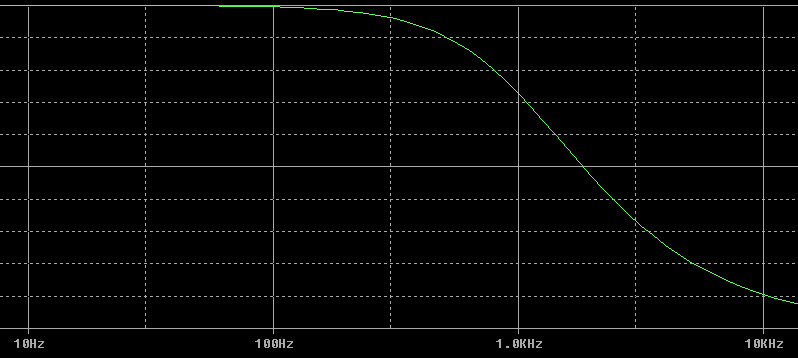
\includegraphics[width=1.0\textwidth]{figures/low_pass_cut_off_frequency1k_150nF.png}
  \caption{Eksempel på low-pass filter med 1k modstand og 1nF kondensator.}
  \label{low_pass}
\end{figure}

%Inde i lys-sensoren sidder der en transistor i en spændingsdeling. Denne transistor kan generere noget høj frekvent støj. Dette filtrers væk med et low-pass filter. 